\chapter{Wstęp}
\label{cha:wstep}

\section{Cel pracy}
\label{sec:celpracy}

Celem pracy jest stworzenie demonstratora systemu wizyjnego do śledzenia obiektów, przy czym zakłada się, że kamera zamontowana jest na głowicy obrotowej. Praca inżynierska obejmuje skompletowanie, we współpracy z opiekunem, stanowiska testowego składającego się z głowicy ruchomej, kamery, platformy obliczeniowej oraz wskaźnika. Należy przeprowadzić analizę oraz weryfikację różnych koncepcji śledzenia, biorąc pod uwagę skuteczność oraz możliwość implementacji sprzętowej lub sprzętowo-programowej. Wybrane rozwiązanie zostanie zaimplementowane, uruchomione i przetestowane w sprzęcie. Wyjście z modułu śledzenia stanowi podstawę do wypracowania pozycjonowania głowicy obrotowej, takiego, aby utrzymać obiekt w środku kadru oraz oznaczyć go wskaźnikiem.

\section{Wprowadzenie}
\label{sec:wprowadzenie}

Automatyczne śledzenie z pomocą kamery jest wykorzystywane m.in. w zagadnieniach związanych z bezpieczeństwem, inwigilacją lub w zastosowaniach wojskowych. Jest ściśle powiązane z wykrywaniem oraz identyfikacją obiektów. Świadczy to o złożoności tego zagadnienia. Śledzenie różni się od innych algorytmów przetwarzania obrazów głównie tym, że musimy wykorzystywać informacje pochodzące z więcej niż jednego kadru. Uwydatnia się to szczególnie, kiedy kamera rejestruje kilka obiektów podobnych do śledzonego. Jeśli zadaniem jest obserwacja jednego konkretnego obiektu, to aby go wyróżnić musimy wykorzystać położenie śledzonego obiektu w poprzednich ramkach \cite{VT}. Znaczące problemy w śledzeniu obiektów mogą być spowodowane zmianą orientacji celu oraz dużą jego szybkością w porównaniu do częstotliwości rejestrowania klatek. W przypadku kamery umieszczonej na głowicy błędy mogą być dodatkowo spowodowane rozmyciem obrazu w trakcie poruszania układu. Istnieją liczne algorytmy służące śledzeniu elementu na obrazach z kamery. Są to m.in:
\begin{itemize}
\item{Śledzenie przez detekcję}
\item{Mean-shift}
%\item{Filtr cząsteczkowy}
\item{KLT}
\end{itemize}
Algorytmy te zostaną dokładniej omówione w kolejnym rozdziale pracy.

\begin{figure}[h]
	\centering
	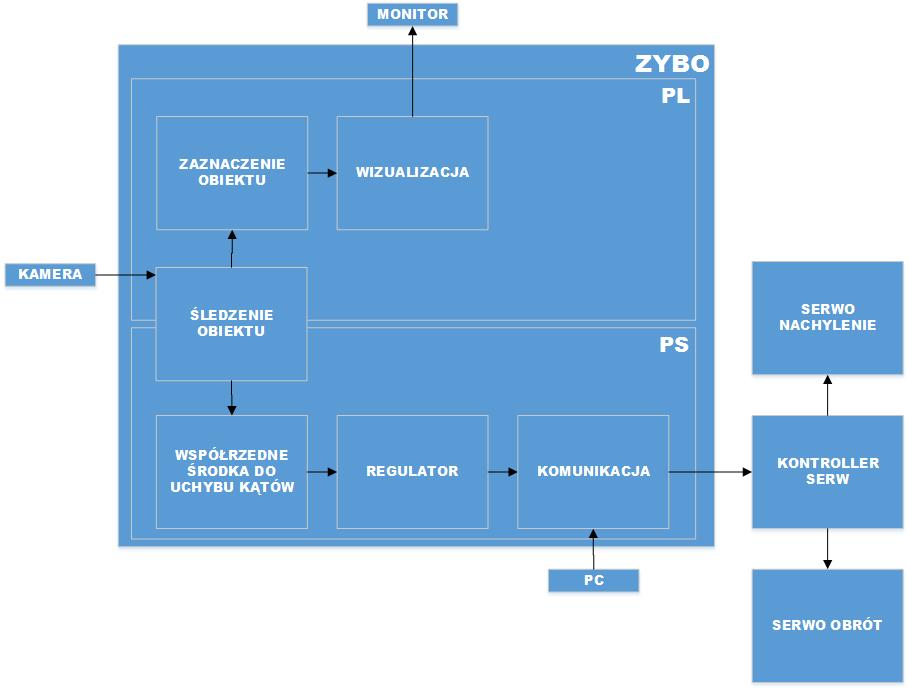
\includegraphics[width=4in]{scheme_pol.jpg}
	\captionsource{Schemat realizowanego rozwiązania.}{Własne}
	\label{fig:schemat}
\end{figure}

\section{Zawartość pracy}
\label{sec:zawartoscpracy}

\subsection{Rozdział 2}
Zrealizowano przegląd algorytmów śledzenia i dokonano wyboru algorytmu do implementacji w sprzęcie.

\subsection{Rozdział 3}
Opisano skompletowane stanowisko. Przedstawiono specyfikację użytych elementów oraz uzasadniono ich wybór.

\subsection{Rozdział 4}
Scharakteryzowano komunikację pomiędzy elementami realizowanego systemu (PC-Zynq-Maestro).

\subsection{Rozdział 5}
Przedstawiono realizację podstawowego toru wizyjnego otrzymującego obraz z kamery i wysyłającego go bez zmian na wyjście.

\subsection{Rozdział 6}
Opisano model matematyczny sterowanego obiektu oraz projekt implementowanego regulatora. Krótko omówiono wynik testu regulatora na modelu.

\subsection{Rozdział 7}
Zrealizowano implementację w platformie sprzętowej gotowego algorytmu Mean-shift, zrealizowanego przez koło naukowe \textit{AVADER}.

\subsection{Rozdział 8}
Przeprowadzono próbę implementacji algorytmu KLT. Opisano działanie modułów odpowiedzialnych za wyznaczanie punktów charakterystycznych obrazu oraz przedstawiono ich działanie na przykładzie.

\subsection{Rozdział 9}
Podsumowano zrealizowane zadania. Omówiono wnioski na podstawie przeprowadzonych prac. Przedstawiono zadania, które zostaną zrealizowane w przyszłości.